\section{Section fine tuning}


\paragraph{Second T}
Regarding the optimization of the second T junction we used the T designed for the previous assignment and we connect to it the two lines routing to the patches. In this way we control also the contributions due to the discontinuities on all the second part of the beam forming network.

\begin{figure}[H]
	\centering
	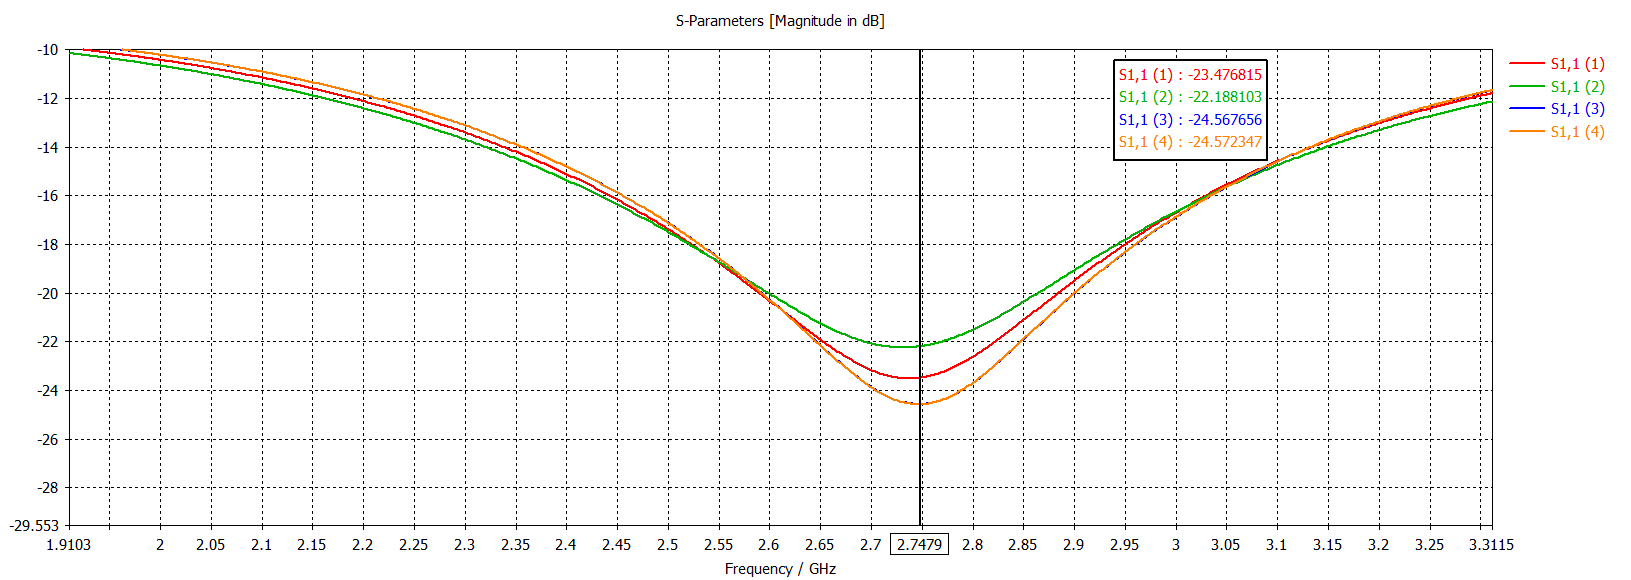
\includegraphics[width=0.9\linewidth]{sT_1angle.png}
	\caption{}
	\label{sT_1angle}
\end{figure}
\begin{figure}[H]
	\centering
	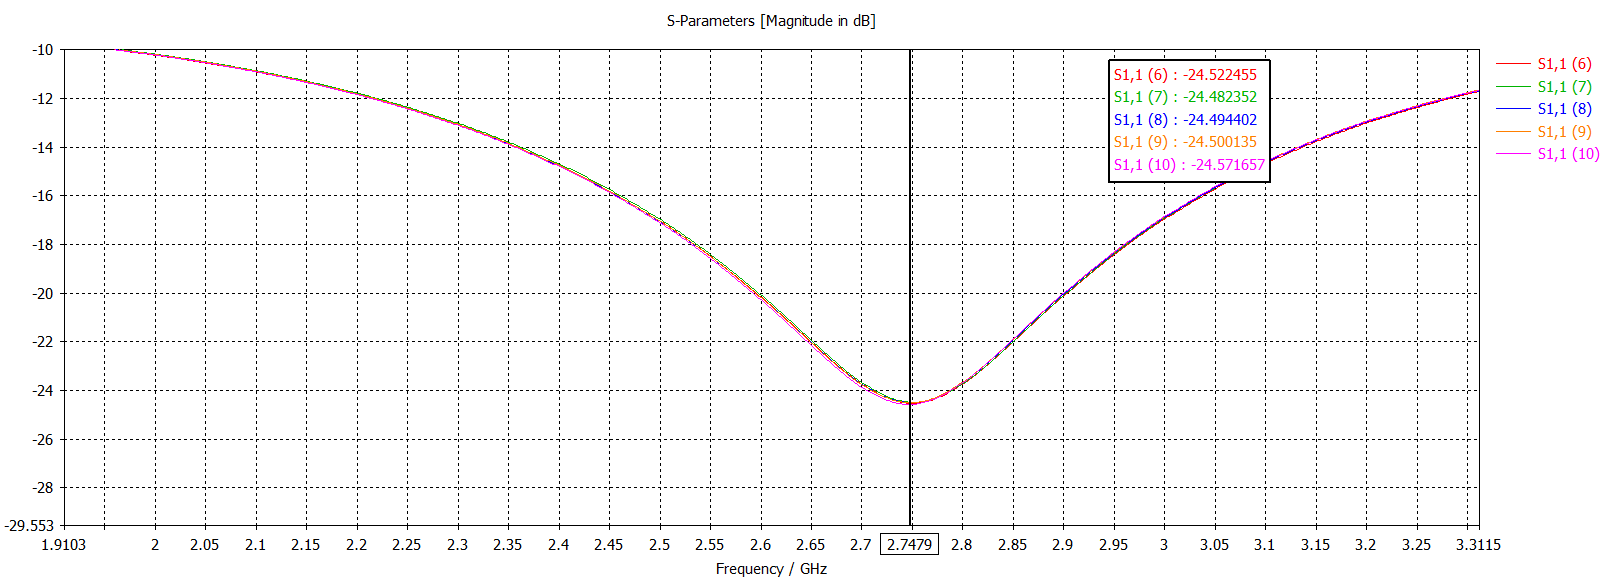
\includegraphics[width=0.9\linewidth]{sT_1depth.png}
	\caption{}
	\label{sT_1depth}
\end{figure}
\begin{figure}[H]
	\centering
	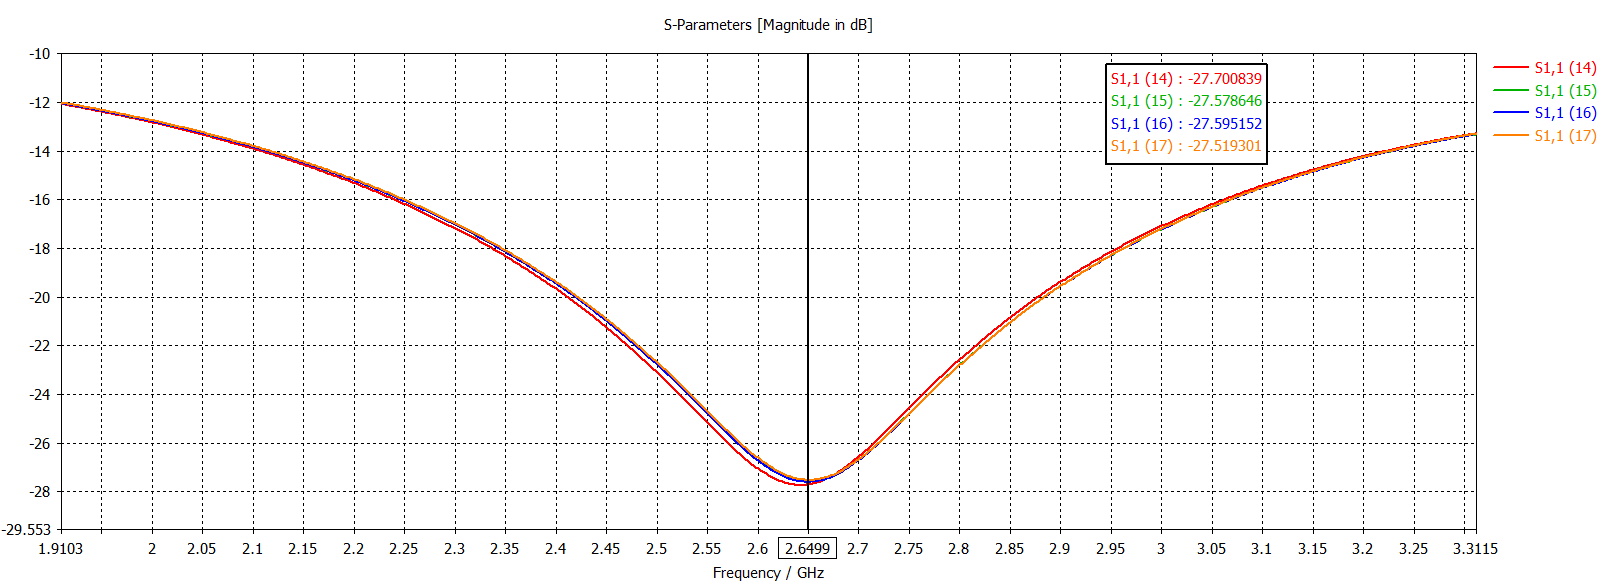
\includegraphics[width=0.9\linewidth]{sT_2depth.png}
	\caption{}
	\label{sT_2depth}
\end{figure}